\section{Object-Oriented GA}
There are many different implementation of Simple Genetic Algorithms(SGA) available. Initially the SGA implementation selected for this project for parallelising was an implementation that closely followed the suggestions of David E. Goldberg's book \textit{"Genetic Algorithms in Search, Optimization, \& Machine learning"} \citep{Goldberg:89}. It was implemented using C++ and took an Object Oriented approach as an abstraction mechanism. There are 37 user modifiable parameters defined to fine tune the behaviour the SGA. It was designed to allow users to change the chromosome structure(haploid or diploid), fixed or variable length chromosome, 3 different mechanism of diploid crossovers, 7 different types of encoding schemes. User could also select fitness function from 15 different implementation(even though only a few of them are actually implemented). It also allows user to select from two different models of elitism, 6 different mechanism of selections. Furthermore, it contains an implementation of Linear Congruential method for generating pseudo random numbers which is used to randomly generate probabilities for mutation and crossover.

This codebase contains over 4,500 lines of code. About 2 weeks time was spent on compiling and running this SGA to understand different parameters and process flow of the algorithm it had implemented. Which was well beyond the planned schedule for this project that is shown in Project plans in Appendix \ref{appendix:project_plans}.

After 2 weeks of studying and experimenting with this SGA implementation, I managed to summarise an analysis of this implementation. this code exhibit many OOD(Object Oriented Development) pitfalls that was common in early Object Oriented Development days. Inheritance was used as a means of implementation reuse without any semantic coherence. Classes are too big and contains too many responsibilities which is against "Single Responsibility principle" of OOD. In many cases, classes violates Liskov's Substitute Principle as well where a derived classes cannot be replaced for the base classes.
Figure \ref{fig:sga_classdiagram} shows the class diagram of this implementation of SGA code using C++.
 

\begin{figure}[!hp]
    \vspace*{-1.5cm}
    \makebox[\linewidth]{
        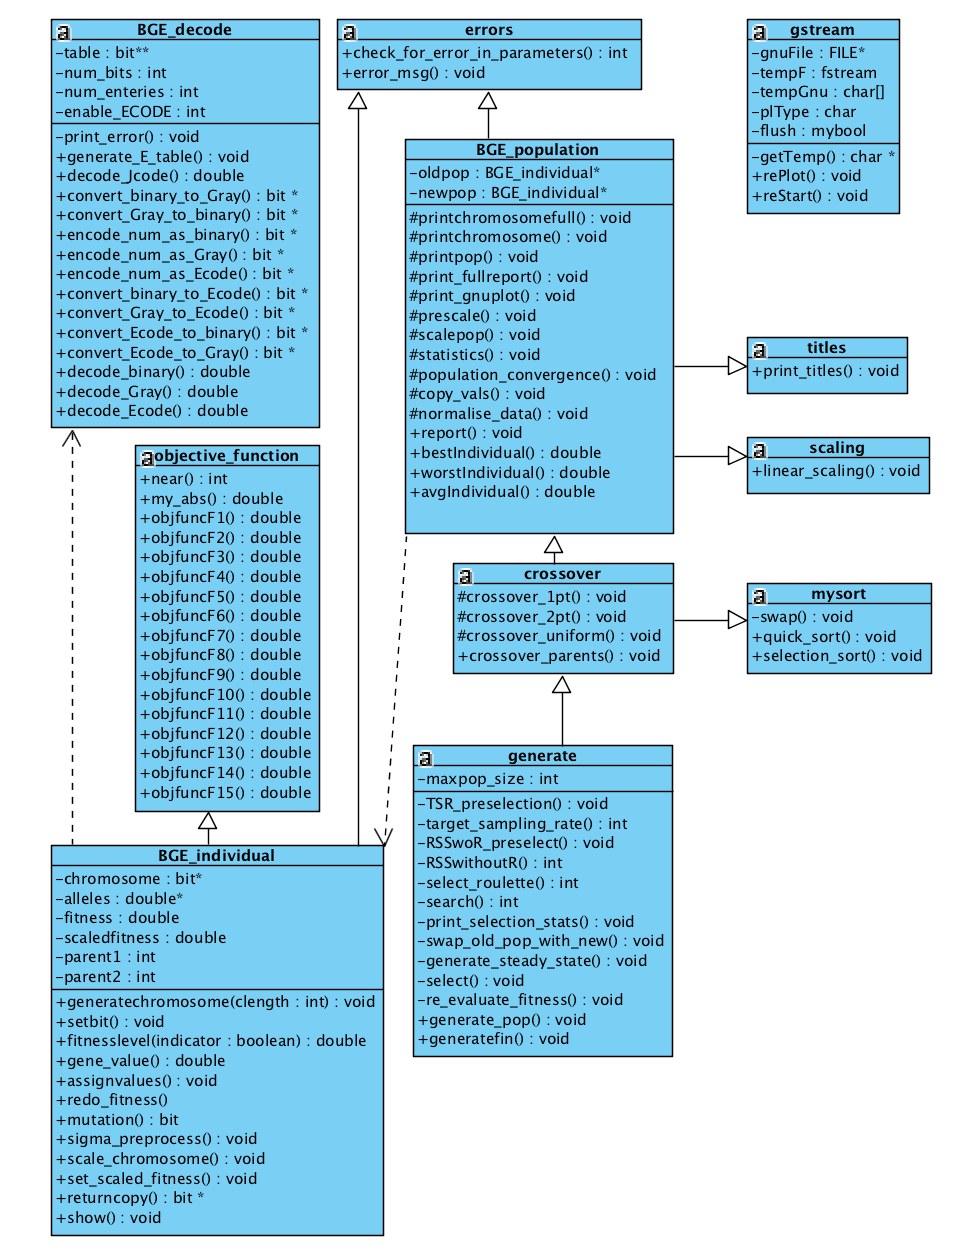
\includegraphics[width=1.3\linewidth]{figs/sga_class_diagram.png}
    }
    \caption{Class diagram of Object-oriented SGA}
     \label{fig:sga_classdiagram}
\end{figure}

\section{Issues with MPI support for Object-oriented paradigm}
The major drawback discovered with object-oriented implementation of GAs was the MPI's lack of support for object-oriented languages. The MPICH 3.2 version of MPI implementation were used this project. With further research on this topic it was discovered none of the major MPI implementation(OpenMPI, ) truly supported the object-oriented C++ other than just the compiler support.

In a conference article titled \textit{"Object Oriented MPI (OOMPI): a class library for the Message Passing Interface"} Squyres et al discussed MPI's lack of support of C++ class libraries and binding. In that paper they suggested an Object Oriented MPI specification \citep{squyresoompi}. However, this effort have been abandoned due to the lack of support from MPI community. After doing further research on this topic in Internet discussion forums and blog posts, it is found that there are ways of doing OO MPI using C++ by using third-party libraries Boost::mpi and Boost::serialization. Boost itself is a set of libraries for the C++ programming language that provide support for tasks and structures such as linear algebra, pseudorandom number generation, multithreading, image processing, regular expressions, and unit testing. Boost is a free to use library licensed under its own free, open-source license, known as the Boost Software License. An MPI program using the Boost::mpi library must initialise an mpi::environment object. This object initialises the MPI environment and enables communication among the processes. This object is initialised with the program arguments in the main program. The creation of this object initialises the MPI environment, and its destruction terminates it. The Boost::mpi requires objects to be serialised so that they are transmissible across processes. The Boost::serialization is a library for serialising C++ objects for sending/receiving data across network. To serialise a class one needs to define a template function serialize() in the class.

There is a little draw back with using Boost::mpi library. The Boost:mpi only implemented MPI1.1 which does not support many useful routines of MPI standards. Some people suggested to use that for regular programs. And for advanced programs to use mainstream MPI-3 libraries with Boost::Serialization for serialising C++ objects. Considering the scope of this project this options is not taken.